\PassOptionsToPackage{top=3cm,left=3cm,right=3cm,bottom=3cm}{geometry}
\documentclass[fleqn,11pt]{wlscirep}

\usepackage{import}
\usepackage{main}

\renewcommand{\paragraph}[1]{\vspace{0.3cm}\noindent\underline{\emph{#1}}\hfill\noindent}

% word count
% \newcommand{\maincount}[1]{%
%   \immediate\write18{texcount -1 -sum=1 -merge -q -nobib #1.tex > #1-words.sum}%
%   \input{#1-words.sum}%
% }

% \newcommand{\abstractcount}[1]{%
%   \immediate\write18{texcount -template="{abst}" #1.tex > #1-words.sum}%
%   \input{#1-words.sum}%
% }

\begin{document}

\doublespacing

\title{\bfseries\LARGE\singlespacing{Transmission of respiratory viral infections with and without air cleaners in a Swiss school under non-pandemic conditions in 2023: A modeling study of epidemiological, environmental, and molecular data}}

% Alternative title: SARS-CoV-2 transmission in schools based on molecular and epidemiological data: potential effects of mask wearing and air cleaners

% author list
\author[1$\ddag$,2]{Nicolas Banholzer}
\author[2,3]{Philipp Jent}
\author[2,4]{Pascal Bittel}
\author[4]{Lavinia Furrer}
\author[4]{Alban Ramette}
\author[4]{Ronald Dijkman}
\author[5]{Jenna Kelly}
\author[1]{Kathrin Zürcher}
\author[1]{Matthias Egger}
\author[2,6]{Tina Hascher}
\author[1*,2]{Lukas Fenner}

\affil[1]{Institute of Social and Preventive Medicine, University of Bern, Bern, Switzerland}
\affil[2]{Multidisciplinary Center for Infectious Diseases, University of Bern, Bern, Switzerland}
\affil[3]{Department of Infectious Diseases, Inselspital, Bern University Hospital, University of Bern, Bern, Switzerland}
\affil[4]{Institute of Infectious Diseases, University of Bern, Bern, Switzerland}
\affil[5]{Interfaculty Bioinformatics Unit, University of Bern, Bern, Switzerland}
\affil[6]{Institute of Educational Science, University of Bern, Bern, Switzerland}


\affil[*]{Corresponding author: lukas.fenner@unibe.ch }

\vspace{1em}

\begin{information}\normalfont

xxxx

% \noindent\textbf{Running head}: SARS-COV-2 transmission in schools and effect of air cleaners

% %\noindent\textbf{Subject categorization}: 6.20  Indoor Air; 10.11 Pediatrics: Respiratory Infections

% \noindent\textbf{Word count}: \maincount{manuscript}words, abstract \abstractcount{manuscript}words (max. 500), title 157 chars (max. 200)

% %\noindent\textbf{Inserts:} 2 tables, 6 figures, 44 references

% \noindent\textbf{S1 Appendix:} Includes supplementary text, tables and figures.

% \vspace{1em}

% \noindent\textbf{Funding}

% \noindent This study is funded by the Multidisciplinary Center for Infectious Diseases, University of Bern, Bern, Switzerland. NB, LF, and ME are supported by the National Institute of Allergy and Infectious Diseases (NIAID) through cooperative agreement 5U01-AI069924-05. ME is supported by special project funding from the Swiss National Science Foundation (grant 32FP30-189498). \medskip

% \noindent\textbf{Contributions}

% \noindent Conception and design: NB, LF. Epidemiological and environmental data collection: NB, PJ, TS, LF. Laboratory data collection: PB, LFu. Additional data collection: TH. Statistical analysis: NB, KZ. Genomic analysis: LB, LFu. Paper draft: NB, LF, ME. All authors reviewed and approved the final version of the manuscript.

% \par
\end{information}

%TC:newcounter abst Words in abstract
%TC:envir abstract [] abst
\begin{abstract}\normalfont
\noindent\textbf{Background:} Airborne respiratory infections can be transmitted in crowded indoor settings, including schools. Infection control measures such as air ventilation or filtration are supposed to reduce the risk of airborne transmission. The aim of this study was to evaluate the real-life effectiveness of portable HEPA-air filtration devices (air cleaners) in reducing the transmission of respiratory viral infections in schools using a multiple-measurement approach. \medskip

\noindent\textbf{Methods and Findings:} We collected epidemiological (absences related to respiratory infections), environmental (CO$_2$ and particle concentrations), and molecular data (bioaerosol and saliva samples) over seven weeks from 16 January to 11 March 2023 in a secondary school (n=38 students in two classes) in Switzerland. We performed laboratory and molecular analyses to detect a panel of 19 respiratory viruses. We installed air cleaners in a cross-over design and compared positive samples and particle concentrations between weeks with and without air filters. We modeled the number of new infections using a Bayesian negative binomial regression model, adjusting for the incubation period, the number of recent and cumulative infections, the ventilation rate, the number of students in class, and community transmission. \\
Molecular analysis detected multiple viruses in saliva samples throughout the study (50/448 positive: 15~influenza B, 15~rhinovirus, 14~adenovirus, 3~SARS-CoV-2, 2~metapneumovirus, and 1~parainfluenza virus), but rarely in bioaerosol samples (2/105 positive: 1~rhinovirus and 1~adenovirus) and on the filters of air cleaners (4/160~positive: 1~influenza~B, 1~HRV, 1~adenovirus, and 1~SARS-CoV-2). The detection rate of positive saliva samples was comparable between study conditions (adjusted relative risk 0.93, 95\%-Credible interval [CrI] 0.49 to 1.61). Daily average CO$_2$ levels were 1,769$\pm$391\,ppm ($\pm$ standard deviation) with air cleaners and 1,636$\pm$341\,ppm without air cleaners, corresponding to similar air change rates (0.74$\pm$0.41\,h$^{-1}$ vs. 0.68$\pm$0.32\,h$^{-1}$). Daily average aerosol number concentrations were 27$\pm$34\,1/cm$^3$ with and 95$\pm$81\,1/cm$^3$ without air cleaners, corresponding to an estimated adjusted decrease of 77\% (95\%-CrI 63\% to 86\%). Absences related to respiratory infections were less frequent with air cleaners in place (13~absences with vs. 21~absences without air cleaners). The estimated risk of infection tended to be lower with air cleaners (adjusted relative risk 0.72, 95\%-Credible Interval 0.44 to 1.15). \medskip 

% Study limitations include unknown specific causes of absences related to respiratory infections (i.e which virus caused the sickness). Furthermore, students occasionally had lessons outside the classroom, thus limiting the potential effectiveness of air cleaners.

\noindent\textbf{Conclusions:} A wide range of non-SARS-CoV-2 respiratory viruses were detected in students, but airborne molecular detection was rare. SARS-CoV-2 was rarely detected in saliva and bioaerosols. Molecular transmission networks documented sustained transmission of non-SARS-CoV-2 seasonal viruses in school rooms despite negative airborne detection, suggesting the need for prolonged close contact. Air cleaners showed a small, potential benefit in reducing airborne transmission. 

\par
\end{abstract}

%TC:ignore

\flushbottom
\maketitle
\setcounter{page}{1}
\thispagestyle{fancy}

\vspace{2em}

%\noindent\textbf{Word count:} \abstractcount{manuscript}words (max. 500)

\vspace{0.5em}

\noindent\textbf{Keywords:} schools, air cleaner, respiratory viruses, airborne transmission, molecular detection
% maximum of 3-5 keywords
\newpage

\sloppy
\raggedbottom
%TC:endignore

\newpage

%TC:break main
\section{Introduction} 

The transmission of respiratory infections such as SARS-CoV-2 and influenza presents significant challenges in terms of mitigation and control. Person-to-person transmission primarily occurs through the release of respiratory particles containing the respective viruses. The recent focus has been on small respiratory particles ($\leq$ 5$\mu$m) called aerosols, which have been found to carry the majority of viruses during respiratory activities\cite{Fennelly2020}. Unlike larger respiratory droplets, which tend to settle quickly, aerosols can remain suspended in the air for several hours and their respiratory plumes can reach more than 2 meters\cite{Coleman2022,Wang2020,Heneghan2021}, exceeding the social distancing rules recommended by public health organizations\cite{Bazant2021PNAS,Trivedi2021PhyFluids,Lindsley2010CID}. 

The generation, spread, and concentration of bioareosols can be influenced by infection control measures. For example, compulsory face mask wearing reduced the transmission of SARS-CoV-2 during the COVID-19 pandemic\cite{Gettings2021,Heinsohn2022,Leech2022PNAS,Mitze2020PNAS,Banholzer2021PLOS}. In addition, improved ventilation systems are critical for a healthy indoor environment both during pandemic and non-pandemic times\cite{Wang2021,Morawska2021}. Portable HEPA-air filtration devices (air cleaners ) may present another cost-effective alternative to upgrading ventilation systems, but the effects of air cleaners on the transmission of respiratory infections are less clear. Various studies showed that air cleaners reduce the concentration of aerosols and particle matter in indoor air\cite{Park2020Build,Buising2022InfContr,Ren2021Dent,Banholzer2023PLoSMed}. These findings suggest potential protection against respiratory infection, as long-term exposure to higher aerosol and particle matter mass concentrations has been associated with increased risk of respiratory infections\cite{Gordon2014Resp} and, more recently, with the incidence and mortality of COVID-19\cite{Kelly2023Atmos,Veronesi2022OccEnvMed,Travaglio2021EnvPoll,DeAngelis2021EnvRes}. Furthermore, a recent study showed that air cleaners effectively removed SARS-CoV-2 bioaerosols in a hospital ward\cite{Morris2022}. Simulation studies have demonstrated the efficacy of air cleaners in reducing the risk of indoor transmission  of SARS-CoV-2\cite{Lindsley2021} and other respiratory viruses\cite{Cortellessa2023Build}.  We have studied the effectiveness of air cleaners in reducing the transmission of SARS-CoV-2 transmission in schools during the pandemic\cite{Banholzer2023PLoSMed}, but the analysis was limited by the study design (installation of air cleaners at the end of the Omicron wave when most students were already infected). In conclusion, empirical evidence linking the use of air cleaners with a reduced risk of infection is lacking. It remains unclear whether reducing particle concentrations and removing bioaerosols from the air will translate in reduced transmission of respiratory infections. 

We used a multiple-measurement approach to study the transmission of viral respiratory viruses and the effect of aircleaners using a cross-over study design in school rooms under non-pandemic conditions in the winter of 2023. We collected epidemiological (absences probably related to respiratory infections), environmental (CO$_2$, aerosol and particle concentrations), and molecular data (detection of respiratory viruses in bioaerosol and human saliva samples) during a seven-week study period from January to March 2022 in two classes of a secondary school in Switzerland. We determined changes in particle concentrations, respiratory virus positivity rates, and modeled the risk of infection.

\newpage

\section{Methods}

\subsection{Study setting and design} 

\noindent We collected data in two classrooms of a secondary school (age of students 14-17~years) in the Canton of Solothurn, Switzerland, over a seven-week study period from 26~January to 11~March 2023. \Cref{fig:study-setup} shows the schematic study setup and Table~\zref{tab:data} in \supp \, provides an overview of the types of data that were collected in each classroom.

\begin{figure}[!htpb]
    \centering
    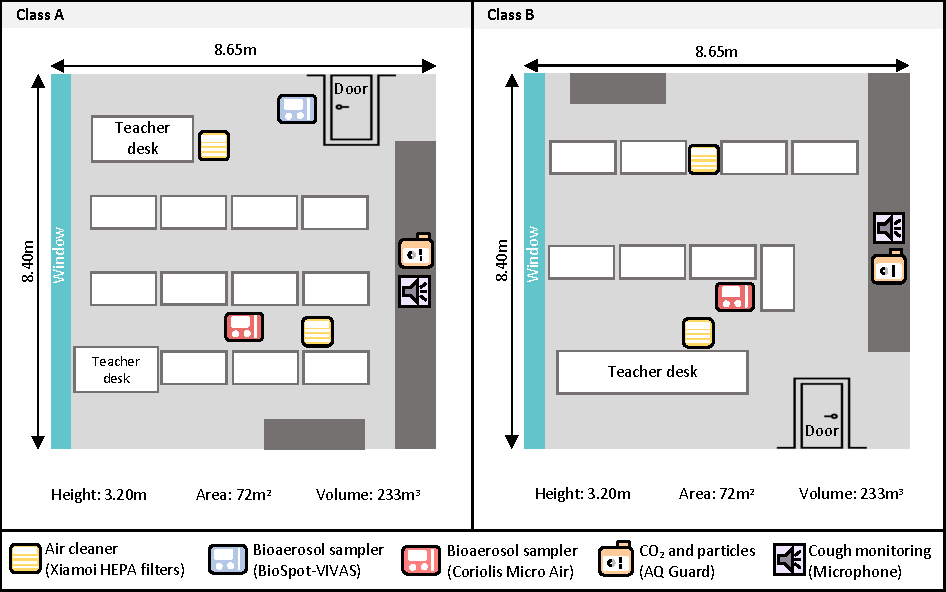
\includegraphics{../study_setting.pdf}
    \caption{\textbf{Study setting}. Schematic study setup of the classrooms. One air cleaner was placed in the front and the other in the back of classrooms. All devices were placed at the head level of students when they were seated. Both classrooms were not equipped with an active HVAC (Heating, Ventilation, Air conditioning) system, but were ventilated using passive window ventilation. }
    \label{fig:study-setup}
\end{figure}

\subsection{Study intervention} 

\noindent We used a cross-over design to study the effectiveness of air cleaners, thereby distinguishing two study conditions in each class: weeks with and weeks without air cleaners being installed in each classroom (\Cref{tab:study_design}). Air cleaners refer to commercially available portable HEPA-filtration devices (Xiaomi Mi Air Pro 70m², Shenzhen, China; approx. USD\,250 per device). According to the manufacturer, these air cleaners run at a clean air delivery rate of 2$\,\times\,$600 m$^{3}$/h. Based on our own experiments conducted in the classrooms, we measured a lower clean air delivery rate of 2$\,\times\,$420 m$^{3}$/h. Window ventilation was done at the discretion of the teachers, as there were no specific recommendations from the national health authorities at that time.

\begin{table}[!htpb]
    \footnotesize
    \centering
    \caption{\textbf{Study design.} Cross-over design where two portable air cleaners (AC) were installed during different time periods in classes A and B over a seven-week study period from 16~January to 11~March 2023, excluding a week of vacation between February 6 and 11. Swabs from the HEPA filters were taken after each intervention phase as indicated by the ``*''.}\label{tab:study_design}
    \begin{tabular}{l l l l l l l l l}
    \toprule
      & \textbf{Week 1} & \textbf{Week 2} & \textbf{Week 3} & Vacation & \textbf{Week 4} & \textbf{Week 5} & \textbf{Week 6} & \textbf{Week 7} \\
      & Jan 16-21 & Jan 23-28 & Jan 30-Feb 3 & Feb 6-11 & Feb 13-18 & Feb 20-25 & Feb 27-March 3 & March 6-11 \\
      \midrule
      \textbf{A} & \cellcolor{gray!50} AC & \cellcolor{gray!50} AC\hphantom{0000}*& \cellcolor{gray!10} None & & \cellcolor{gray!10} None & \cellcolor{gray!10} None & \cellcolor{gray!50} AC & \cellcolor{gray!50} AC\hphantom{00009}* \\
      \textbf{B} & \cellcolor{gray!10} None & \cellcolor{gray!10} None & \cellcolor{gray!50} AC\hphantom{0000000}* & & \cellcolor{gray!50} AC & \cellcolor{gray!50} AC\hphantom{0000}*& \cellcolor{gray!10} None & \cellcolor{gray!10} None \\
      \bottomrule
    \end{tabular}
\end{table}
 
\subsection{Data collection}

\noindent\textbf{Epidemiological data} \smallskip

\noindent At the beginning of the study, we collected aggregated data on age, sex and COVID-19 vaccination and recovery status in the participating classes. Daily we collected data on each absent student, \ie the absence and return date as well as the reason for the absence (sickness, career days,  or other). For sickness-related absences, we collected the symptoms and the symptom onset date. We also collected data on laboratory tests but none of the students reported a test result over the study. Based on the epidemiological data, we defined a case of respiratory infection as an absence where the student reported a sickness with at least one of the following symptoms: fever, coughing, tiredness, loss of test or smell, sore throat, headache, aches and pains, diarrhea, difficulty breathing or shortness of breath, stomach. Students were asked to report the first date when they experienced symptoms, \eg a student absent on Monday can also report Saturday or Sunday as the symptom onset date. We will denote respiratory cases by their symptom onset date, which usually corresponded to the absence date, unless the student went to school while having symptoms. Informed consent of one student could not be obtained and the sole absence of this student was considered as unrelated to a respiratory infection. Reports about absences were entered electronically into a REDcap database\cite{Harris2009,Harris2019}. The line list data is shown in Table~\zref{tab:epi-data-line-list} in \supp. 

In addition, both classes participated in repetitive bi-weekly (Tuesdays and Thursdays) testing for a panel of respiratory infections (see \nameref{sec:mol_analyses} below). The saliva samples were transported to the laboratory and stored at $-$80°C until further processed\cite{Galar2021,To2019,Huber2021}. The line list data is shown in Table~\zref{tab:mol-data-line-list} in \supp. \medskip

\noindent\textbf{Environmental data} \smallskip

\noindent \emph{CO$_2$ and particle measurements} 

\noindent An air quality device (AQ Guard, Palas GmbH, Karlsruhe, Germany) continuously measured indoor CO$_2$ levels, aerosol number concentrations (particle diameter between 175~nm to 20~$\mu$m) and particle mass concentrations (PM; PM$_1$, PM$_{2.5}$, PM$_4$, PM$_{10}$) by minute. This device has been used in previous work\cite{DiGilio2021,Duill2021,Banholzer2023PLoSMed}. A transient mass balance model was used to estimate the air change rate from indoor CO$_2$ levels\cite{Batterman2017IJERPH}, assuming that the classrooms were fully occupied during lessons and that room occupancy increased (decreased) linearly 10~minutes before (after) the start (end) of a lesson. Particle concentrations were filtered according to the times students were in the classroom, which were monitored together with the times during which windows were opened. \medskip

\noindent \emph{Bioaerosol sampling and HEPA filters of the air cleaners} 

\noindent We collected airborne respiratory viruses in both classrooms with a bioaerosol sampling device (Coriolis Micro Air, Bertin Instruments Montigny-le-Bretonneux, France) , running at 200\,l/min and collecting into 15\,mL PBS, as previously reported in clinic settings\cite{Moore2021}. The Coriolis Micro Air only operated shortly before and during break times to reduce noise exposure (approximately 60\,min/day). In one class, we also used the BioSpot-VIVAS device sampler (Aerosol Devices Inc., Ft. Collins, CO, USA). This device samples airborne virus particles into a viral transport medium (VTM) using a laminar flow water-based condensation method\cite{Pan2016JAM,Lednicky2016AST}. BioSpot-VIVAS operated throughout lessons. The removable parts of both sampling devices were regularly autoclaved to avoid contamination. At the end of the day, samples were transported to the Institute of Infectious Diseases (IFIK) and stored at $-$80°C. After each intervention phase (see \Cref{tab:study_design}), the HEPA filters were carefully removed from the air cleaners, divided into 20~fields, and one swab per field was taken for a total of 20~swabs per filter.\medskip

\subsection{Laboratory and molecular analyses}\label{sec:mol_analyses}

\noindent Prior to the real-time (RT)-PCR analysis, daily bioaerosol samples were combined for each sampling device and filtered using Amicon Ultra-15 Centrifugal Filters with Ultracel 10,000 Dalton molecular weight cutoffs filters (UFC9010; MilliporeSigma, Burlington, USA) to a volume of 1\,mL. The human saliva samples were directly analyzed without prior filtration. The Allplex RV Master Assay (Seegene, Seoul, South Korea) detects a panel of 19~respiratory viruses: SARS-CoV-2, Influenza A virus, Influenza B virus, Human respiratory syncytial virus A/B (RSV), Human metapneumovirus (MPV), Human adenovirus A/B/C/D/E/F (AdV), Human rhinovirus A/B/C (HRV), and Human parainfluenza virus 1/2/3/4 (PIV) in one single reaction. %/Viral genome load (VGL) of specimens was quantified (copies/L) by curve extrapolation derived from standardized ATCC quantitative genomic standard dilutions (ATCC-VR-3347D, LGC Standards, LGC Group UK). For the BioSpot-VIVAS air samples, the air concentration of the DNA was exactly calculated according to the airflow influx into the sampling device. %/ 
The Limit of detection (LOD) of the assay SARS-CoV-2, IFA/IFB is 7.5x10$^0$ TCID/ml (SARS-CoV-2), 3.7x10$^{-1}$ TCID/ml (IFA), and 4.8x100 TCID/ml (100cp/ml) (IFB) respectively.
For positive samples, we performed targeted sequencing to compare genetic relatedness between SARS-CoV-2 strains detected in the air and human samples\cite{Goncalves2021Microorganisms}, but we were unable to amplify and sequence any of the gene targets in the bioaerosol samples due to low RNA concentrations. 

\subsection{Molecular genotyping}

For adenovirus-positive samples (saliva, bioaerosol, and air filter samples), we used a PCR procedure to amplify three hypervariable regions of the viral genome and then sequenced the PCR products\cite{Akello2020ClinicEpi}. The phylogenetic trees were constructed using the Neighbor-Joining method based on evolutionary distances computed using the number of differences method. The molecular transmission network for influenza B was determined by whole genome sequencing\cite{Kelly2022FrontiersImmuno}.

\subsection{Audio recordings and cough detection}

We installed one microphone (RØDE NT-USB; Sydney, Australia) in each classroom to continuously record sounds. We detected the number of coughs per minute using an AI algorithm based on a convolutional neural network\cite{Bertschinger2023IEEE}, which was recently trained and validated with audio data from the waiting room of a primary care clinic\cite{Zurcher2022}. 

\subsection{Statistical analyses and modeling}

All statistical analyses were described in the statistical analysis plan (SAP)\cite{Banholzer2023SAP}, which was published before analyses began. In contrast to the SAP, the number of positive bioaerosol samples and the viral load concentration of positive samples could not be analyzed because there were too few positive samples over the study. Apart from that there were no major deviations from the SAP regarding the conducted analyses. There were a few minor deviations from the SAP (\eg small changes in prior distributions or model specifications), which are documented in Supplementary Text~\zref{sec:transmission-model} to Supplementary Text~\zref{sec:env-regression-model} in \supp, which provide detailed descriptions of the models used in each analysis.

\noindent\textbf{Risk of infection} \smallskip

\noindent We estimated the relative risk of infection with air cleaners using a Bayesian latent hierarchical regression model. The observed outcome of this model is the number of new respiratory cases $C$ (absences related to respiratory infections by date of symptom onset) on day $t$ in class $j$, which are modeled with a Negative Binomial distribution. The expected number of new cases is the weighted sum of the number of new infections $I_{js}$ (unobserved/latent outcome) in the previous days $s<t$, with the weights corresponding to the probability distribution of the incubation period. The number of new infections is related to the presence of air cleaners using a regression-like log-link
\begin{align}
    \log I_{js} = \log F_{js} - \log N_{js} + \beta_0 + \beta_1 \cdot \text{AirCleaner}_{js},
\end{align}
where $F_{js}$ is the number of infections in the previous week (a proxy for the number of infectious students), $N_{js}$ is the cumulative number of infections, $\beta_0$ is the infection rate without air cleaners, and $\beta_1$ is the effect of air cleaners. Furthermore, the effect of air cleaners is adjusted for class-specific effects, the number of students in class, the daily air change rate, and the weekly positivity rate for COVID-19 and the consultations for influenza-like illnesses in the community (\ie the Canton of Solothurn).

A detailed description of the model and choice of priors for all model parameters are provided in Supplementary Text~\zref{sec:transmission-model} in \supp. Importantly, since multiple viruses were prevalent over the study period, we considered the distribution of the incubation period to be a weighted mix of the virus-specific distributions. The weights were inferred based on the proportion of positive saliva samples for each virus per week. As a result, the distribution of the incubation period used for modeling could change every week depending on the proportion of viruses that were detected in the students' saliva. Moreover, respiratory cases by date of symptom onset were under-reported for weekends and thus a re-weighting scheme was used to account for weekday effects. \medskip

\noindent\textbf{Number of positive saliva samples} \smallskip

\noindent Molecular analysis determined which saliva samples were positive for a respiratory virus. We analyzed the number of positive saliva samples with a Bayesian Multinomial logistic regression model (Supplementary Text~\zref{sec:multinomial-model} in \supp) where the expected number of positive samples for a virus was linked to the presence of air cleaners, adjusting for class-specific effects and the number of susceptibles for each virus. The latter was computed as the difference between the number of students per class and the cumulative number of positive samples. As a sensitivity analysis, we lagged the test results by one test date (\ie from Tuesday to last Thursday and from Thursday to Tuesday) and one test week (\ie from Tuesday to last Tuesday and Thursday to last Thursday), to consider the unknown delay when students were infected and tested positive. \medskip

\noindent\textbf{Aerosol and particle concentrations} \smallskip

\noindent We computed the average concentrations per day and compared these between study conditions. We estimated the reduction in concentrations using Bayesian log-linear regression models (Supplementary Text~\zref{sec:env-regression-model} in \supp), adjusting for class and weekday effects, the number of students in class, the air change rate, and the cumulative number of respiratory cases. \medskip

\noindent\textbf{Number of detected coughs} \smallskip

\noindent We computed the daily number of detected coughs and compared it between study conditions. We estimated the reduction in the number of coughs using a Bayesian Negative Binomial regression model (Supplementary Text~\zref{sec:aud-regression-model}) with time in class as the model offset, adjusting for class and weekday effects, the number of students in class, the air change rate, and the cumulative number of respiratory cases. In addition, we used a Bayesian Negative Binomial hierarchical (random effects) regression model to estimate the association between the number of coughs and the number of positive saliva test results for respiratory viruses. For this analysis, we only used the days were saliva testing was performed and coughs could be detected because people were in the classroom (27~days in total).  \medskip


\noindent\textbf{Software and model estimation} \smallskip

\noindent All analyses were performed in R software (version 4.2.0)\cite{RCoreTeam2022} and modeling in Stan (version 2.21.0)\cite{Carpenter2017}. Model parameters were estimated with a Bayesian approach. Specifically, Markov chain Monte Carlo (MCMC) sampling was used as implemented by the Hamiltonian Monte Carlo algorithm with the No-U-Turn Sampler (NUTS)\cite{Hoffman2014}. Each model is estimated with 4 Markov chains and 2,000 iterations of which the first 1,000 iterations are discarded as part of the warm-up. Estimation power is evaluated via the effective sample size ESS and convergence of the Markov chains is evaluated with the Gelman-Rubin convergence diagnostic ($\hat{R}$). If not stated otherwise, we report posterior means and credible intervals (CrIs) based on the 50\%, 80\%, and 95\% quantiles of the posterior samples, respectively. The code is available from \url{https://osf.io/38j9g}.

% \subsection{Additional data collection} 

% \noindent We also collected data about the students' subjective experiences of well-being and emotions using standardized daily online questionnaires and a pre-post questionnaire\cite{Brandenberger2018}. These data are not part of the current analysis. 

\subsection{Ethics statement}

\noindent The Ethics Committee of the Canton of Bern, Switzerland, approved the study (reference no. 2021-02377). For the saliva samples, we included all students who were willing to participate and obtained written informed consent from their caregivers.


\newpage

\section{Results}

The study population consisted of 38~students (19~female, 19~male; Table~\ref{tab:cases-overview-school}). Of these, 7~students were vaccinated or recovered from an infection within SARS-CoV-2 in the last four months. Over the seven-week study period (1,330 student-days in total), students were absent from school for 220~days (18\% of total) of which 129~days (59\% of absences) were due to sickness.  

\begin{table}[!htpb]
    \centering
    \caption{Overview of the study population and person-days of absences.}
    \label{tab:cases-overview-school}
    \footnotesize
    \begin{tabular}{l r r r}
    \toprule
         &  Class A & Class B & Total \\ \midrule 
        \textbf{Students} & \textbf{20 (53\%)} & \textbf{18 (47\%)} & \textbf{38 (100\%)} \\
        \emph{Gender} \\
        $\drsh$ Female & 11 (55\%) & 8 (44\%) & 19 (\hphantom{0}50\%) \\
        $\drsh$ Male & 9 (45\%) & 10 (56\%) & 19 (\hphantom{0}50\%) \\
        \emph{Immunity status} \\
        $\drsh$ Recently vaccinated (or recovered) & 7 (39\%) & 0 (0\%) & 7 (\hphantom{0}18\%) \\
        $\drsh$ Not recently vaccinated (or recovered) & 11 (61\%) & 20 (100\%) & 31 (\hphantom{0}82\%) \\
        \textbf{Absent person-days} & \textbf{110 (50\%)} & \textbf{110 (50\%)} & \textbf{220 (100\%)} \\
        $\drsh$ Sickness & 52 (47\%) & 77 (70\%) & 129 (\hphantom{0}59\%) \\
        $\drsh$ Other & 58 (53\%) & 33 (30\%) & 91 (\hphantom{0}41\%) \\
        \bottomrule
    \end{tabular} 
\end{table}

\subsection{Molecular analyses}

We analyzed 448~saliva samples over the study across classes. We detected 15~influenza~B~(Flu B), 15~rhinoviruses~(HRV), 14~adenovirus (AdV), 3~SARS-CoV-2~(CoV), 2~metapneumoviruses~(MPV), and 1~parainfluenza~virus~(PIV) (\Cref{fig:molecular-descriptives}a). There was an equal number of positive samples with and without air cleaners (\Cref{fig:molecular-descriptives}b). Taking into account the number of samples and the number of suceptible students, the positivity rate remained comparable between study conditions (adjusted relative risk 0.93, 95\%-Credible interval [CrI] 0.49 to 1.61), and was not sensitivity to infection to testing delays (Figure~\zref{fig:mol-estimation-results-sensitivity} in \supp). The distribution of positive samples varied between classes (\Cref{fig:molecular-descriptives}c). For example, in the first three study weeks all except for one sample were positive for AdV in class~A, while the vast majority of positive Flu~B samples were found in class~B. The virus-specific variations between classes are suggestive of transmission occurring within classes. Accordingly, we have manually labeled possible transmission chains within classes as shown in \Cref{fig:molecular-network}.

We also analyzed 105~bioaerosol samples and detected  two respiratory viruses in the air (1~HRV in class~A and 1~AdV in class~B). Furthermore, we detected 1~Flu~B, 1~HRV, 1~AdV, and 1~CoV in the 20~swabs taken from each filter of an air cleaner after each intervention phase (160~swabs in total).


\begin{figure}[!htpb]
    \centering
    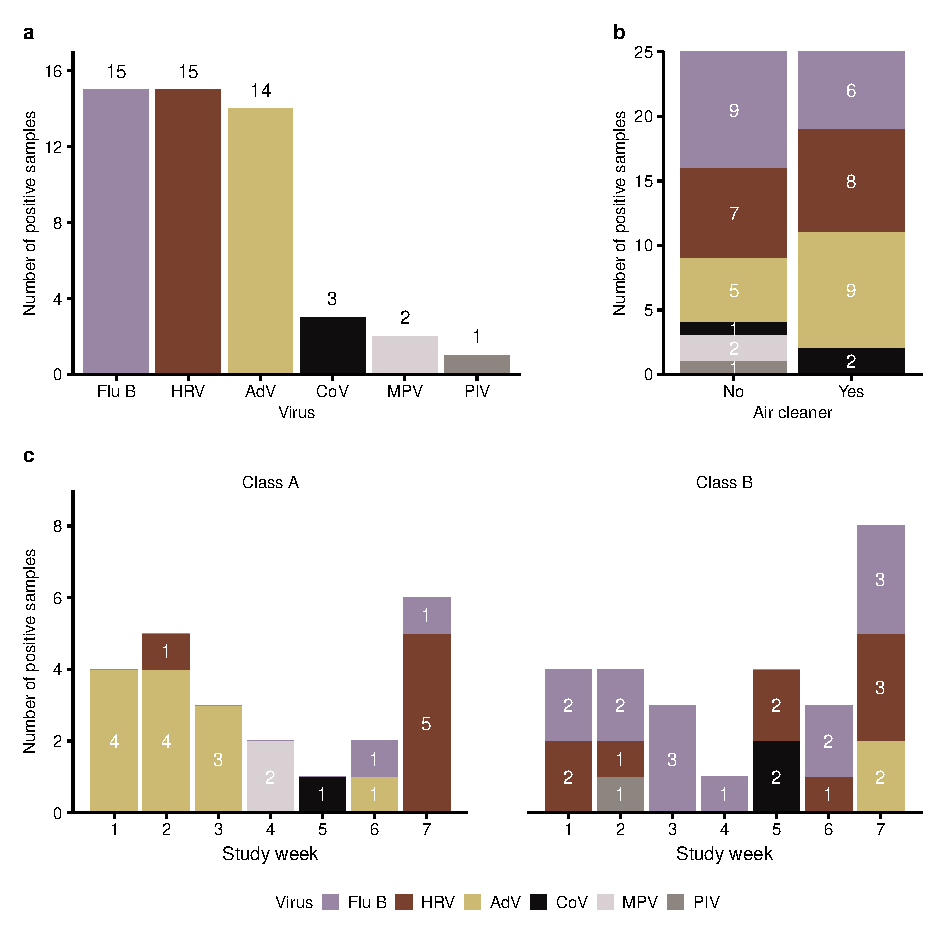
\includegraphics{../../results/mol-data/descriptives.pdf}
    \caption{\textbf{Analysis of molecular data}. Number of positive saliva samples by \textbf{(a)}~virus, \textbf{(b)}~study condition, and \textbf{(c)}~study week and class. Flu B: Influenza B, HRV: rhinovirus, AdV: adenovirus, CoV: SARS-CoV-2, MPV: metapneumovirus, PIV: parainfluenza virus.}
    \label{fig:molecular-descriptives}
\end{figure}


\begin{figure}[!htpb]
    \centering
    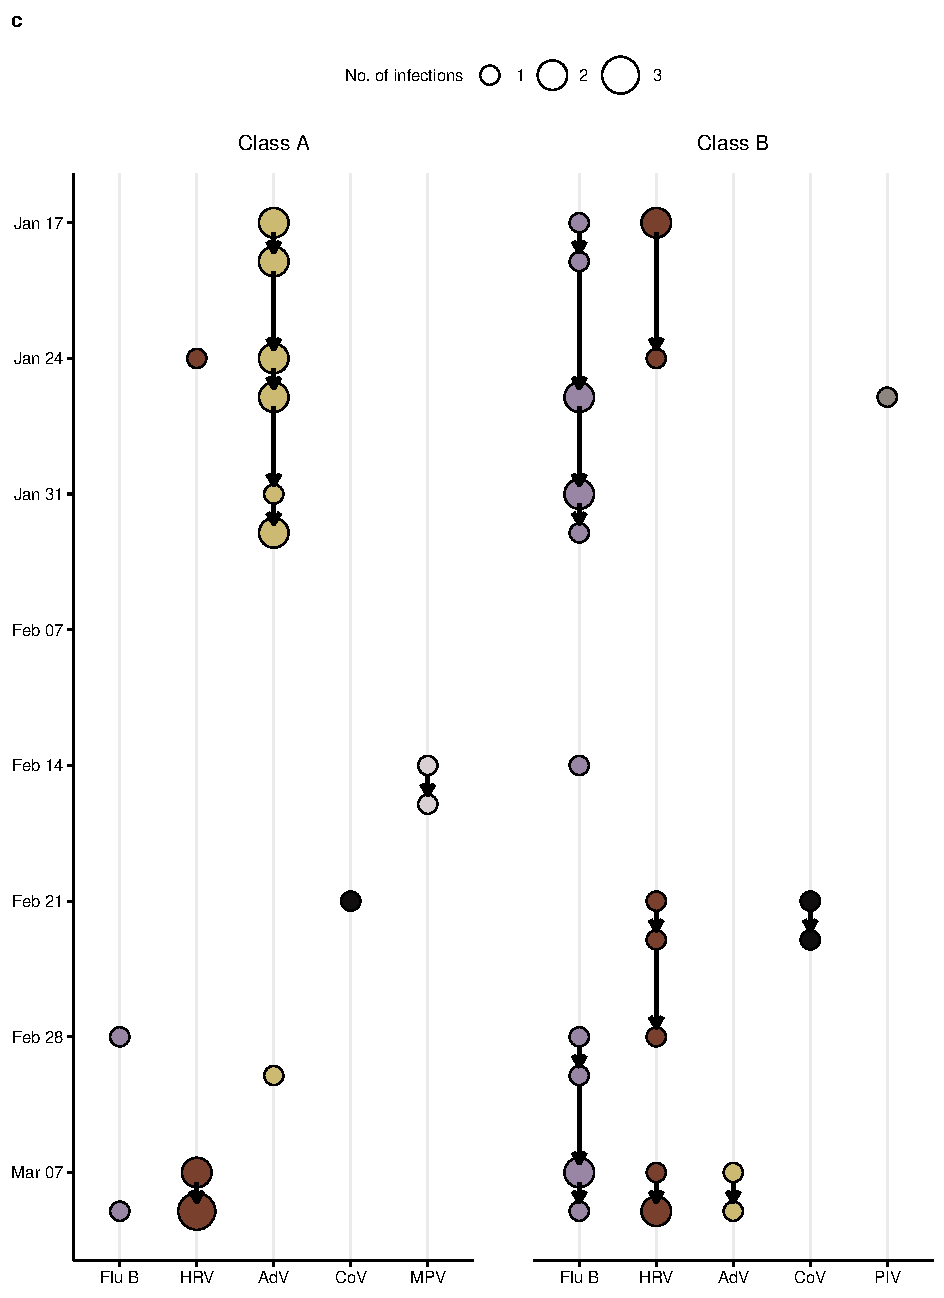
\includegraphics{../../results/mol-data/network-plot.pdf}
    \caption{\textbf{Transmission network}. Daily number of positive saliva samples (dot sizes) and possible transmission chains within classes (directed arrows). Positive samples are linked if they are of the same virus and less than 1~week apart. Flu B: Influenza B, HRV: rhinovirus, AdV: adenovirus, CoV: SARS-CoV-2, MPV: metapneumovirus, PIV: parainfluenza virus.}
    \label{fig:molecular-network}
\end{figure}

\subsection{Analysis of aerosol and particle concentrations}

There was a strong difference in particle concentrations between study conditions (\Cref{fig:palas-results}a). Aerosol number concentration with air cleaners were markedly lower (27$\pm$34\,1/cm$^3$) than without air cleaners (95$\pm$81\,1/cm$^3$). Similarly, particle mass concentrations (\eg PM$_1$) were markedly lower with air cleaners (1.16$\pm$1.33\,$\mu$gm$^{-3}$) than without air cleaners (4.20$\pm$3.74\,$\mu$gm$^{-3}$). There was no considerable difference in other environmental variables (Figure~\zref{fig:env-descriptives-other-vars} in \supp). In particular, daily average CO$_2$ levels (air change rates) were 1,769$\pm$391\,ppm (0.74$\pm$0.41\,h$^{-1}$) with air cleaners and 1,636$\pm$341\,ppm (0.68$\pm$0.32\,h$^{-1}$), suggesting that ventilation was comparable between study conditions. When adjusting for air change rates and multiple other factors, the aerosol number concentration decreased by 76\% (95\%-CrI 63\% to 86\%) with air cleaners (\Cref{fig:palas-results}b and Table~\zref{tab:palas-est-results} in \supp). The decrease in the concentration of larger particles (PM$_{10}$) was larger than the decrease in the concentration of smaller particles (PM$_1$ to PM$_{4}$). 

\begin{figure}[!htpb]
\centering
    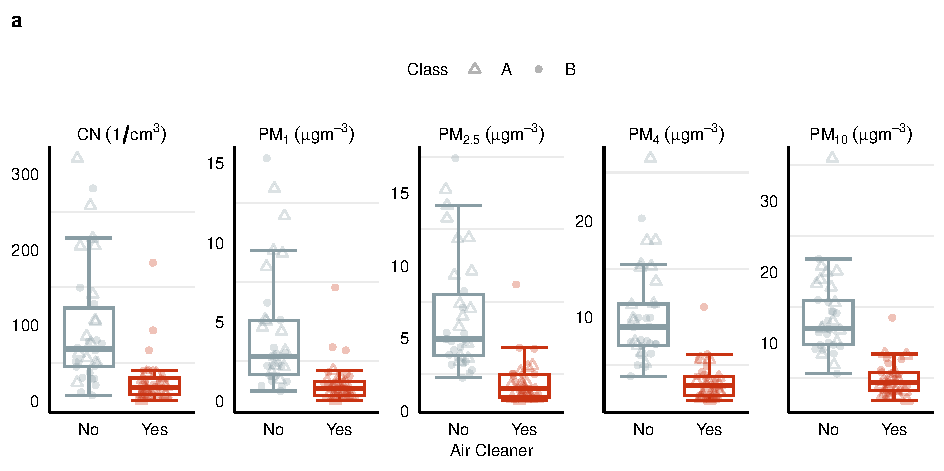
\includegraphics[width=\linewidth]{../../results/env-data/particles-boxplot.pdf}
    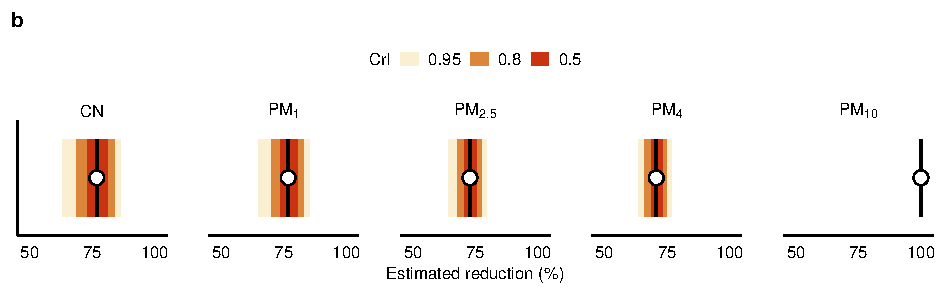
\includegraphics[width=\linewidth]{../../results/env-data/estimation-results-figure.pdf}
    \caption{\textbf{Analysis of particle concentrations and comparison between study conditions}. \textbf{(a)}~Boxplot of the daily average values for aerosol number concentration (CN in 1/cm$^3$) and particle mass concentration (PM for particles of sizes <1 to <10~$\mu$m, respectively in $\mu$gm$^{-3}$). \textbf{(b)}~Estimated reduction in aerosol number and particle mass concentrations with air cleaners (posterior mean as dot and 50\%-, 80\%- and 95\%-CrI as lines, respectively). }
    \label{fig:palas-results}
\end{figure}

\subsection{Risk of infection}

Overall, there were 35~respiratory cases (absences related to respiratory infections) across classes. Incidentally, there were more cases in class~B (21) than in class~A (14), which is the class were more students recently recovered from a SARS-CoV-2 infection or were vaccinated. Except for one study week, there was an equal or higher number of cases without air cleaners (\Cref{fig:redcap-results}a). Based on our Bayesian latent hierarchical regression model, we estimated a trend towards a lower risk of infection with air cleaners (adjusted relative risk 0.72, 95\%-Credible Interval 0.44 to 1.15). As a result, the estimated number of infections if air cleaners had been installed throughout the study is expected to be 36 (95\%-CrI 21 to 64) compared to 62 (95\%-CrI 29 to 141) infections if they would not have been installed (\Cref{fig:redcap-results}b). Detailed estimation results are provided in Supplementary Text~\zref{sec:detailed-redcap} in \supp. 

\begin{figure}[!htpb]
    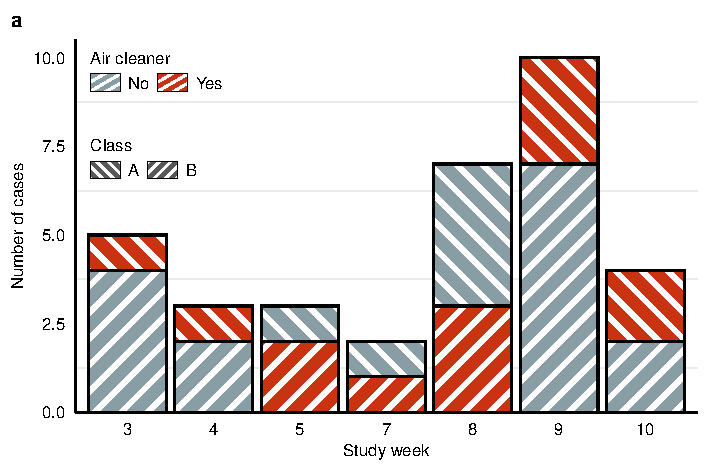
\includegraphics[width=\linewidth]{../../results/epi-data/cases_by_week.pdf} 
    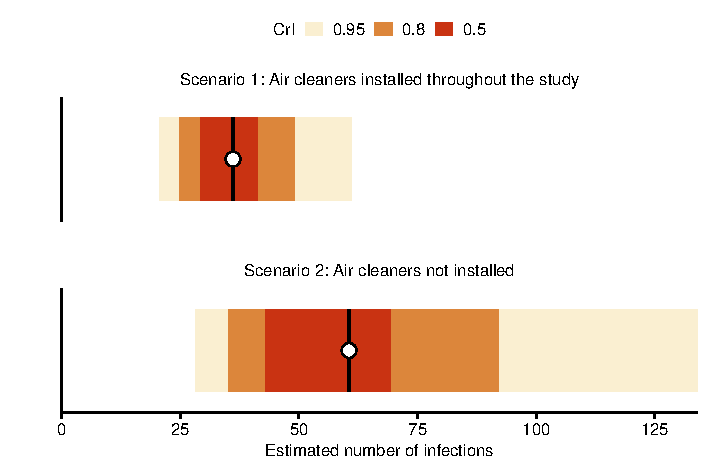
\includegraphics[width=\linewidth]{../../results/epi-data/avoided-infections.pdf}
    \caption{\textbf{Analysis of epidemiological data and estimated number of infections with and without air cleaners.}. \textbf{(a)}~Weekly number of respiratory cases with and without air cleaners. \textbf{(b)}~Estimated mean number of infections (posterior mean as dot and 50\%, 80\%, and 95\%-CrI as shaded areas) if, in both classes, air cleaners had been installed throughout the study or not been installed.}
    \label{fig:redcap-results}
\end{figure}

\subsection{Detected coughs}

Slightly fewer coughs were detected during study weeks where air cleaners were installed (\Cref{fig:coughing}a). On average, there were 2.5~coughs/min with and 3.1~coughs/min without air cleaners (adjusted relative risk 0.93, 95\%-CrI 0.85 to 1.02). Significantly more coughs were detected in class~B (adjusted relative risk 2.16, 95\%-CrI 1.90 to 2.46), suggesting a link with the observed variation in virus-specific transmission between classes (\Cref{fig:molecular-descriptives}c). This link can also be seen in the association between the frequency of coughing and the number of positive saliva tests for respiratory viruses (\Cref{fig:coughing}b). Coughing was more frequent for Flu~B (relative risk 1.25, 95\%-CrI 1.03 to 1.53) and slightly less frequent with AdV (0.87, 95\%-CrI 0.49 to 1.12). 

\begin{figure}[!htpb]
    \centering
    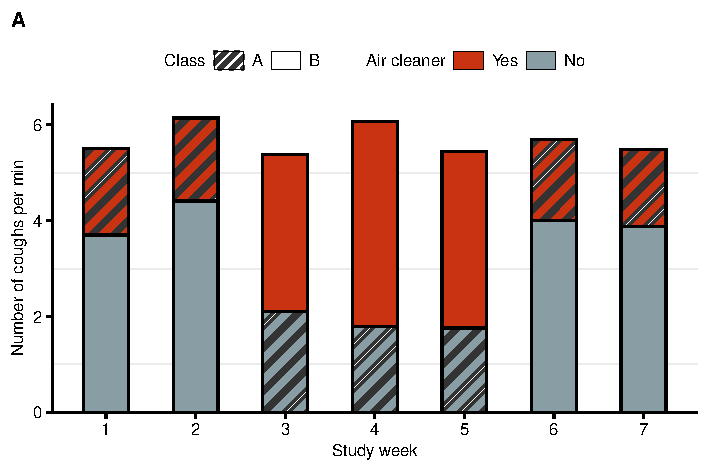
\includegraphics{results/cough-data/coughs-frequency-per-week.pdf}
    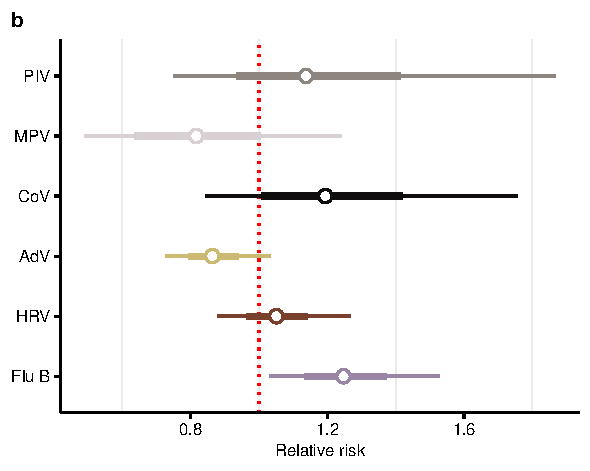
\includegraphics{results/cough-data/coughs-virus-association.pdf}
    \caption{\textbf{Analysis of coughing data.} \textbf{(a)}~Daily average number of detected coughs per minute by study week, condition and class. \textbf{(b)}~Estimated association (relative risk; posterior mean as dot, 50\%, 80\%, and 95\%-CrI as lines) between cough frequency and number of positive saliva test results by respiratory virus.}
    \label{fig:coughing}
\end{figure}

\subsection{Comparison with previous study}

In a previous study\cite{Banholzer2023PLoSMed}, we estimated the effectiveness of mask wearing and air cleaners during the SARS-CoV-2 Omicron wave. \Cref{fig:comparison} shows a comparison of the results. The distribution of respiratory infections is different (\Cref{fig:comparison}a) because we almost exclusively detected SARS-CoV-2 in our previous study during the COVID-19 pandemic, as compared to a range of respiratory infections in this study during non-pandemic times. Although there were more positive saliva samples in this study, the number of respiratory infections detected in bioaerosols and on the HEPA-filters of the air cleaners was lower (\Cref{fig:comparison}b).
The reductions in particle concentrations were larger and with lower uncertainty in this study (\Cref{fig:comparison}c). The risk of infection tended to be lower with air cleaners in this study where air cleaners were analyzed using a cross-over design, but not in our previous study where air cleaners were installed only at the end of the study when most students had already been infected with SARS-Cov-2(\Cref{fig:comparison}d).

\begin{figure}[!htpb]
    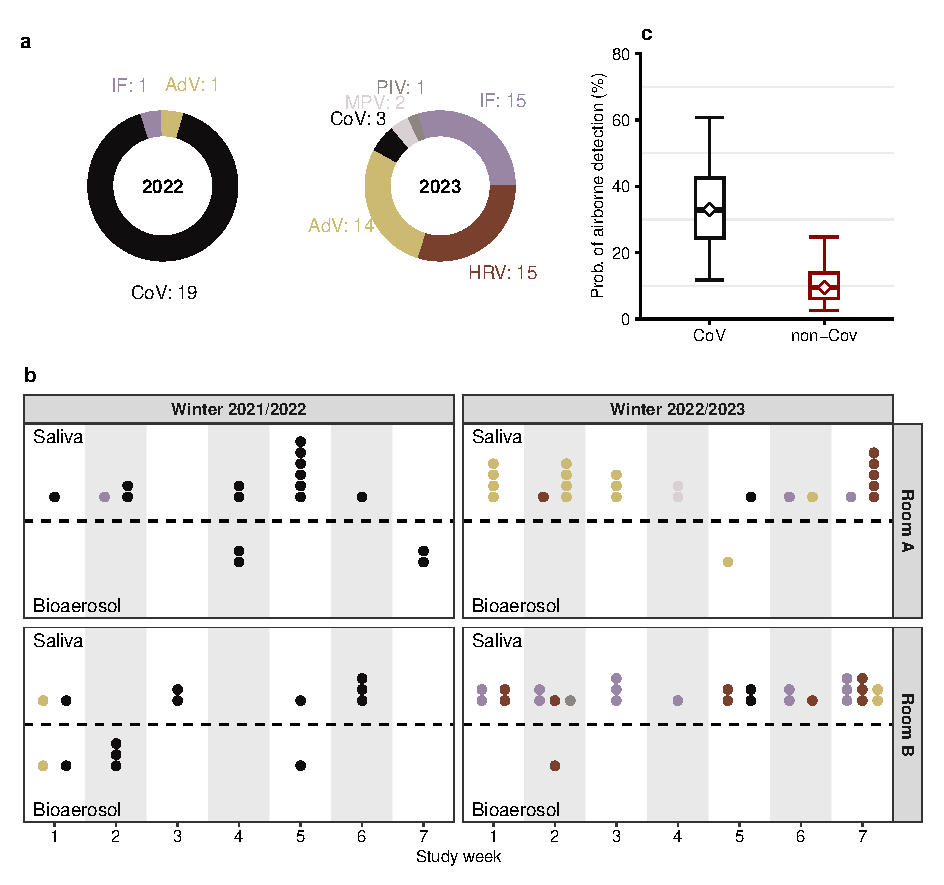
\includegraphics[width=\linewidth]{../../results/comparison.pdf} 
    \caption{\textbf{Comparison of the results between our previous study in 2022 during the COVID-19 pandemic (blue) and this study in 2023 during non-pandemic times (black).}. \textbf{(a)}~Proportion of positive saliva samples and virus. Viruses: Influenza B (Flu B), rhinovirus (HRV), adenovirus (AdV), SARS-CoV-2 (CoV), metapneumovirus (MPV), parainfluenza virus (PIV). \textbf{(b)}~Number of positive saliva, bioaerosol, and HEPA-filter samples. \textbf{(c)}~Estimated reduction in aerosol number and particle mass concentrations (CN in 1/cm$^3$) and particle mass concentration (PM for particles of sizes <1 to <10~$\mu$m, respectively in $\mu$gm$^{-3}$) with air cleaners (posterior mean as squares and 95\%-CrI as lines). \textbf{(d)}~Adjusted relative risk of infection (posterior mean as squares and 95\%-CrI as lines).}
    \label{fig:comparison}
\end{figure}


\FloatBarrier

\newpage

\section{Discussion}

% summary

We collected epidemiological, environmental, and molecular data to estimate the risk of infection with respiratory viruses in a Swiss school and assessed the effectiveness of air cleaners as an infection control measure. We found a wide range of respiratory viruses in human saliva samples, primarily adenovirus, influenza B, and rhinovirus, but only few non-SARS-CoV-2 respiratory viruses were detected in bioaerosol samples and on the filters of air cleaners. Aerosol number and particle mass concentrations decreased significantly with air cleaners and Bayesian modeling based on the absences of students showed a small reduction in the relative risk of infection with air cleaners. Reduced intensity of symptoms (coughing) in school, as determined by acoustic recording, indicates small prevention of symptomatic infections by air cleaners.

% comparison with our previous study

In a previous study\cite{Banholzer2023PLoSMed}, we estimated the effectiveness of mask wearing and air cleaners in reducing the transmission of SARS-CoV-2 in two Swiss schools. We only found a detectable effect on the risk of infection for mask wearing, but not air cleaners. We argued that air cleaners may have had less potential to reduce infections because they were implemented at the end of the study when most students had already been infected with SARS-CoV-2. In this study, we used a cross-over design to estimate the effectiveness of air cleaners again, but this time under non-pandemic conditions. We found similar reductions in particle concentrations and a tendency that the relative risk of infection was lower with air cleaners. To some extent, the differences between the two studies may be explained by different adjustments. While we could not adjust for ventilation in our previous study, the estimates of this study were adjusted for the daily air change rate, which correlated with the relative risk of infection (see Supplementary Text~\zref{sec:detailed-molecular} in \supp). Furthermore, the distribution of respiratory viruses in this study was very different from the distribution in our previous study. 

% why could we not detect so many bioaerosols

We detected fewer respiratory viruses in bioaerosol samples compared to our previous study\cite{Banholzer2023PLoSMed} (1~sample of adenovirus and 1~sample of rhinovirus in this study vs 10~samples of SARS-CoV-2 in the previous study), especially in relation to the number of positive saliva samples (50~samples in this study vs 21~in the previous study). Similarly, the number of viruses detected on the filters of the air cleaners was also lower in this study (4~positive samples in 160~swabs vs 8~positive samples in 80~swabs in the previous study). Importantly, there was a clear shift in the distribution of respiratory viruses in the current study compared to the previous study in 2022 during the SARS-CoV-2 Omicron variant. Whereas in 2022 we detected almost exclusively SARS-CoV-2 in human saliva, the most common respiratory viruses in 2023 were adenovirus, influenza~B, and rhinoviruses (only three SARS-CoV-2-positive samples). The shift in the pattern of respiratory viruses has been observed in other studies\cite{Nygaard2023Lancet,Sauteur2022EuroSurv}. 

% other reasons

Technical reasons for the differences in airborne detection are unlikely. The bioaerosol sampling devices and laboratory procedures were the same in both studies and no technical issues were observed. Instead, airborne detection could have been influenced by environmental factors. Although temperature (overall between 19 and 25$^{\circ}$C) and relative humidity (overall between 25 and 50\%) were similar in both studies, the same levels can have a different effect on airborne survival of respiratory viruses. For example, for rhinovirus and adenovirus, survival increases with relative humidity, while the reverse relationship has been documented for influenza and SARS-CoV-2\cite{Tellier2009JTRSI,Ahlawat2020AAQR,Biryukov2020mS,Karim1985CJM,Davis1971AM}. A change in ventilation conditions could have had a profound effect, but CO$_2$ levels were even higher in this study (1,702$\pm$370\,ppm vs 1,064$\pm$232\,ppm in the previous study), suggesting that classrooms were not as well ventilated as during the COVID-19 pandemic. Although lower ventilation was partially offset by a greater reduction in aerosol and particle concentrations from air cleaners, the removal of particles through air cleaners may be slower than through ventilation.

% bioaerosol sampling in more depth

As a consequence, we speculate that the difference in airborne molecular detection of respiratory viruses is due to the characteristics of the respiratory viruses. Differences in physicochemical properties of virus-laden aerosols (\eg physical size, viral load, and infectivity), which influence the generation and survival of airborne viral RNA\cite{Wang2021,Sattar2016Book}, could make it easier to detect SARS-CoV-2 in the air. The reason is that viral loads do often not exceed the detection limits of existing devices for bioaerosol sampling, which remains a challenge\cite{Wang2021,Belser2023PLOSPath,Bekking2019IORV,Mainelis2020AST}. For example, one study was unable to detect any human rhinovirus in the exhaled breath of 16~HRV-infected subjects\cite{Fabian2011JAMPDD}. Nevertheless, previous studies show that also influenza\cite{Bischoff2013JID,Pan2017mSphere}, rhinovirus\cite{Myatt2004AJRCCM}, and adenovirus\cite{Nguyen2017OFID,Pan2017mSphere} can be detected in airborne samples. The ability to detect pathogens in bioaerosols could also be related to patient characteristics of the study participants. Multiple studies suggest an association between the generation of pathogenic aerosols and infectiousness\cite{Leung2020NatMed,Bischoff2013JID,Escombe2008PLoSMed}. Therefore, studies including more infectious patients (intentionally or unintentionally) will probably have a higher chance of detecting respiratory viruses in the air. 

% transmission within classrooms

The low rate of positive bioaerosol samples also means that it is unclear to what extent students airborne transmission occurred in classrooms. It may be possible that students had rather little exposure to respiratory viruses in schools and acquired their infections elsewhere. However, the distribution of saliva samples between classes shows remarkable differences. For example, adenovirus was spreading entirely in class~A in the first three study weeks and only two infections with influenza~B occurred over the study. By contrast, influenza~B was spreading throughout the study in class~B and infections with adenovirus were only detected in the last study week. Adenovirus infections often tend to be mild\cite{Kunz2010CIDR} and less associated with coughing than influenza\cite{Ma2018RMV}, which is in line with the comparably lower frequency of detected coughs in class~B. Altogether, the class-specific patterns in the spread of respiratory viruses indicate that transmission of respiratory infections may have occurred at least to some extent within the classrooms. 

% effects of air cleaners

Our study indicated a small, potential benefit of air cleaners, but other infection control measures such as universal mask wearing appear to be more effective\cite{Banholzer2023PLoSMed,Heinsohn2022,Gettings2021,Dharmadhikari2012AJRCCM,Leung2020NatMed,Milton2013PLoSPathogens}. There may be several reasons for this. Compared to \eg mask wearing, air cleaners cannot influence transmission outside the classrooms. Furthermore, previous work suggests that prolonged close contact may be needed for transmission\cite{Leung2020NatMed,Brankston2007LancetID}, or make transmission more likely despite prior vaccination or infection\cite{Lind2023NatCommun}. However, compared to face masks, air cleaners are unable to prevent such close range high particle density aerosol transmission. Evidence from our previous\cite{Banholzer2023PLoSMed} and this study further suggest that air cleaners are more effective in the removal of larger particles ($>5\mu$m). Yet, a larger proportion of respiratory viruses are carried in the smaller particles ($\leq5\mu$m)\cite{Fennelly2020}. Finally, classroom activity, airflow and other unobserved, confounding factors make it difficult to assess the effects of air cleaners. Nevertheless, it is important to assess their effectiveness in a real-life setting, and compare with the hypothetical impact suggested by simulation studies\cite{Lindsley2021,Cortellessa2023Build}.


% limitations

Our study has several limitations. First, aerosol measurements and molecular detection of viruses in bioaerosol samples document exposure, but not necessarily transmission and the direction of transmission (human to air, air to human) cannot be determined. Nevertheless, the virus-specific distribution of positive saliva samples between classes indicate potential transmission within classrooms. Second, it was not possible to ascertain the specific causes for the absences based on the epidemiological data. Therefore, some absences may have falsely been attributed to respiratory infections and we could only approximate the incubation period for each epidemiological case. Third, the effectiveness of air cleaners was somewhat limited because students occasionally had lessons outside the classroom. This is in contrast to other infection control measures such as face masks that had to be used in every indoor space during pandemic times.

% conclusion

In conclusion, using epidemiological, environmental, and molecular data, our study shows that considerable transmission of respiratory viruses other than SARS-CoV-2 occurred in school rooms under non-pandemic conditions. Air cleaners significantly reduced aerosol concentrations, but airborne respiratory viruses were rarely detected, suggesting that prolonged close contact may be required for transmission. The epidemiologic transmission model estimated a tendency towards lower transmission with air filters. Future studies may use our multiple-measurement approach to assess whether professional building ventilation, which should be preferred over air cleaners in the long term, and other infection control measures reduce the risk of airborne transmission. Whether their effectiveness varies with the seasonal distribution of respiratory viruses under non-pandemic conditions also remains to be investigated. 


\newpage


%TC:ignore
\section*{Acknowledgements}
We would like to thank the schools, teachers, and students participating in the study. We are grateful to the Educational Department of the Canton of Solothurn for their support throughout the study. We also would like to thank the biosecurity team at the Institute for Infectious Diseases of the University of Bern for their assistance with the bioaerosol devices (Kathrina Summermatter, Julia Feldmann, and Monika Gsell). Finally, we are indebted to the student assistants who helped with the data collection at the schools.

\bibliography{references.bib}
%TC:endignore

\end{document}
